% Options for packages loaded elsewhere
\PassOptionsToPackage{unicode}{hyperref}
\PassOptionsToPackage{hyphens}{url}
%
\documentclass[
]{book}
\usepackage{lmodern}
\usepackage{amssymb,amsmath}
\usepackage{ifxetex,ifluatex}
\ifnum 0\ifxetex 1\fi\ifluatex 1\fi=0 % if pdftex
  \usepackage[T1]{fontenc}
  \usepackage[utf8]{inputenc}
  \usepackage{textcomp} % provide euro and other symbols
\else % if luatex or xetex
  \usepackage{unicode-math}
  \defaultfontfeatures{Scale=MatchLowercase}
  \defaultfontfeatures[\rmfamily]{Ligatures=TeX,Scale=1}
\fi
% Use upquote if available, for straight quotes in verbatim environments
\IfFileExists{upquote.sty}{\usepackage{upquote}}{}
\IfFileExists{microtype.sty}{% use microtype if available
  \usepackage[]{microtype}
  \UseMicrotypeSet[protrusion]{basicmath} % disable protrusion for tt fonts
}{}
\makeatletter
\@ifundefined{KOMAClassName}{% if non-KOMA class
  \IfFileExists{parskip.sty}{%
    \usepackage{parskip}
  }{% else
    \setlength{\parindent}{0pt}
    \setlength{\parskip}{6pt plus 2pt minus 1pt}}
}{% if KOMA class
  \KOMAoptions{parskip=half}}
\makeatother
\usepackage{xcolor}
\IfFileExists{xurl.sty}{\usepackage{xurl}}{} % add URL line breaks if available
\IfFileExists{bookmark.sty}{\usepackage{bookmark}}{\usepackage{hyperref}}
\hypersetup{
  pdftitle={A tutorial for geochemical modeling of fluid-rock interaction using GEM-Selektor and the MINES thermodynamic database},
  pdfauthor={Alexander Gysi},
  hidelinks,
  pdfcreator={LaTeX via pandoc}}
\urlstyle{same} % disable monospaced font for URLs
\usepackage{longtable,booktabs}
% Correct order of tables after \paragraph or \subparagraph
\usepackage{etoolbox}
\makeatletter
\patchcmd\longtable{\par}{\if@noskipsec\mbox{}\fi\par}{}{}
\makeatother
% Allow footnotes in longtable head/foot
\IfFileExists{footnotehyper.sty}{\usepackage{footnotehyper}}{\usepackage{footnote}}
\makesavenoteenv{longtable}
\usepackage{graphicx,grffile}
\makeatletter
\def\maxwidth{\ifdim\Gin@nat@width>\linewidth\linewidth\else\Gin@nat@width\fi}
\def\maxheight{\ifdim\Gin@nat@height>\textheight\textheight\else\Gin@nat@height\fi}
\makeatother
% Scale images if necessary, so that they will not overflow the page
% margins by default, and it is still possible to overwrite the defaults
% using explicit options in \includegraphics[width, height, ...]{}
\setkeys{Gin}{width=\maxwidth,height=\maxheight,keepaspectratio}
% Set default figure placement to htbp
\makeatletter
\def\fps@figure{htbp}
\makeatother
\setlength{\emergencystretch}{3em} % prevent overfull lines
\providecommand{\tightlist}{%
  \setlength{\itemsep}{0pt}\setlength{\parskip}{0pt}}
\setcounter{secnumdepth}{5}
\usepackage{booktabs}
\usepackage{amsthm}
\makeatletter
\def\thm@space@setup{%
  \thm@preskip=8pt plus 2pt minus 4pt
  \thm@postskip=\thm@preskip
}
\makeatother
\usepackage[]{natbib}
\bibliographystyle{apalike}

\title{A tutorial for geochemical modeling of fluid-rock interaction using GEM-Selektor and the MINES thermodynamic database}
\author{Alexander Gysi}
\date{2020-09-21}

\begin{document}
\maketitle

{
\setcounter{tocdepth}{1}
\tableofcontents
}
\hypertarget{prerequisites}{%
\chapter*{Prerequisites}\label{prerequisites}}
\addcontentsline{toc}{chapter}{Prerequisites}

GEM-Selektor (GEMS), is a numerical modeling program with a graphical user interface based on Gibbs energy minimization and permits calculating and solving fluid-rock interaction problems of interest in geochemistry.

\begin{itemize}
\item
  Installation instructions for GEMS and more information about this modeling program can be found on the GEMS team webpage: \url{http://gems.web.psi.ch/GEMS3/techinfo.html}.
\item
  Information about the MINES database and project files for the tutorials can be found under \url{https://geoinfo.nmt.edu/tdb}
\end{itemize}

This booklet is subdivided into five modules.

\begin{itemize}
\tightlist
\item
  Module 1: Create your first project in GEMS and installing the MINES database
\end{itemize}

\hypertarget{intro}{%
\chapter{Create your first project in GEMS}\label{intro}}

Here we will learn how to create a new Project, the selection of thermodynamic databases, components and equations of state for your modeling project. We will also explain the project folder structure and how to install the \href{https://geoinfo.nmt.edu/tdb}{MINES thermodynamic database} for modeling hydrothermal fluid-rock interaction and ore-forming processes . You will also learn how to interact basalt with water in your first equilibrium calculations.

\hypertarget{installing-the-mines-thermodynamic-database}{%
\section{Installing the MINES thermodynamic database}\label{installing-the-mines-thermodynamic-database}}

The MINES thermodynamic database can be downloaded at \url{https://geoinfo.nmt.edu/tdb} (Fig. \ref{fig:fig-1}).

\begin{figure}
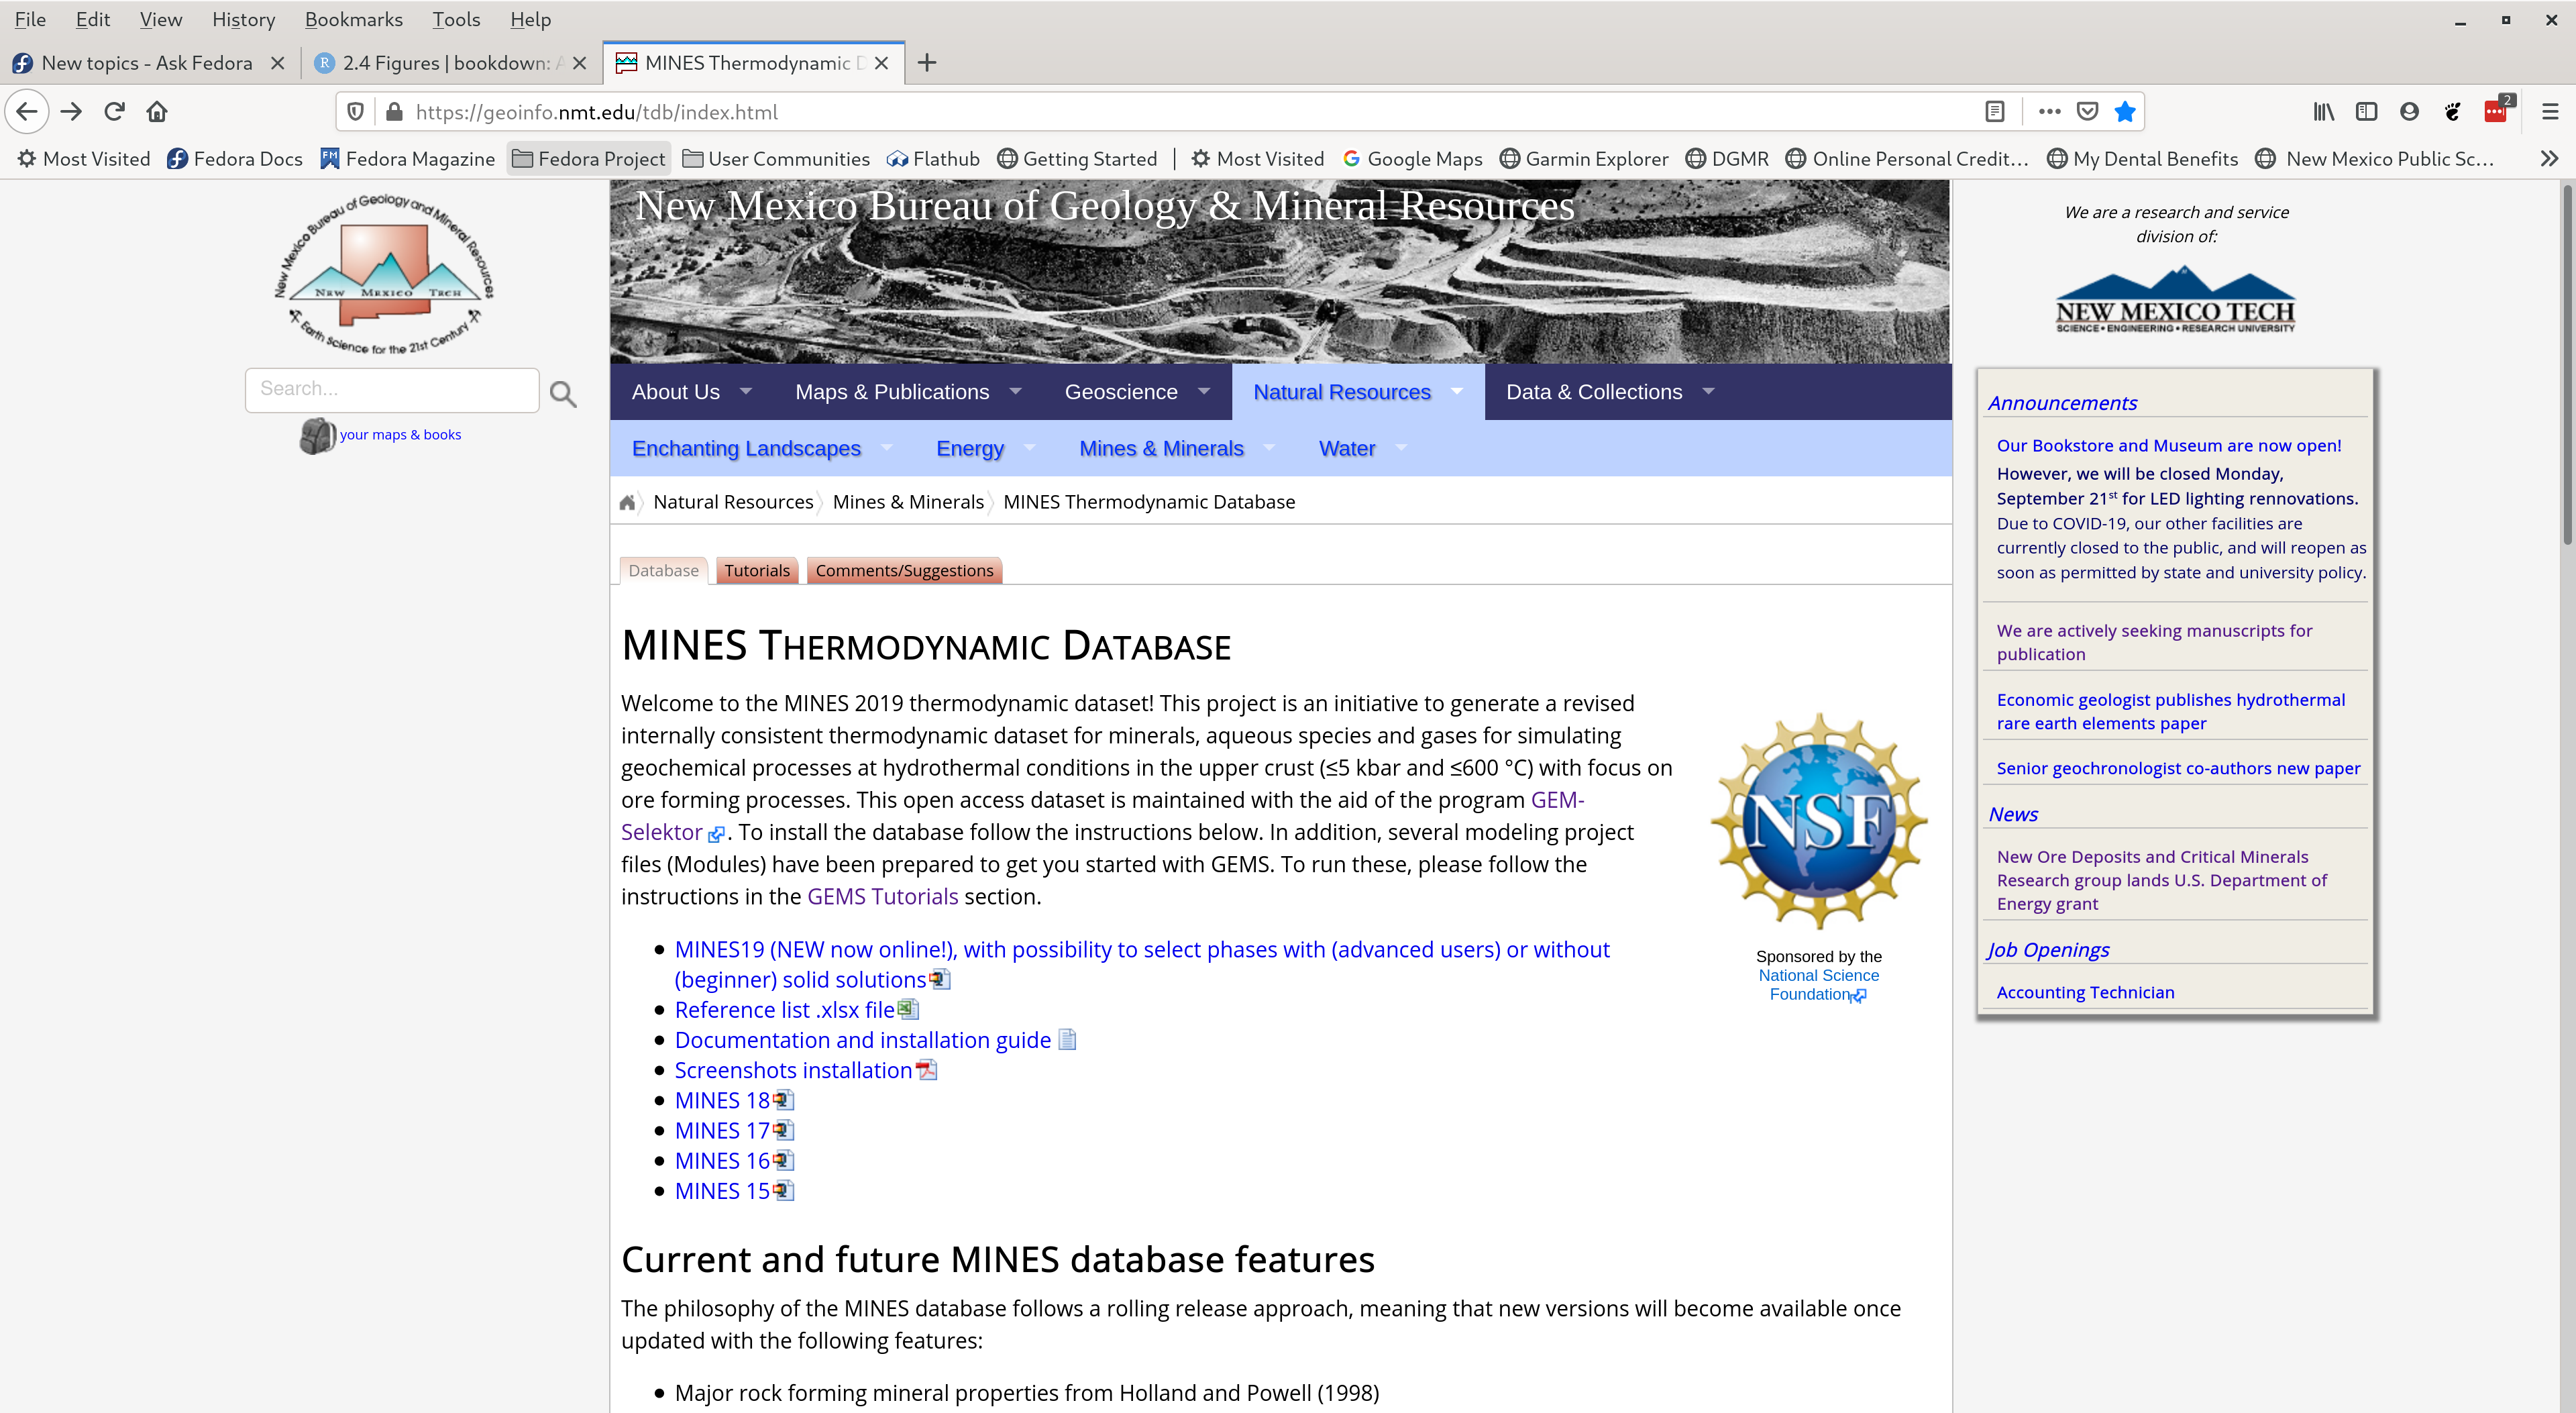
\includegraphics[width=0.9\linewidth]{figures/module1/fig-1} \caption{The MINES thermodynamic database webpage and files to download. Select the weblink for MINES19.}\label{fig:fig-1}
\end{figure}

\begin{itemize}
\item
  Download and unzip the DB19.default archive folder to Downloads. Select all the database files in this folder and copy them (Fig. \ref{fig:fig-2}).
\item
  Merge these database files with the Gems3-app/Resources/DB.default folder by pasting them into DB.default (Fig. \ref{fig:fig-3}).
\end{itemize}

\emph{In Linux this folder is in /Gems3-app/Resources/DB.default; In Mac OSX this folder is in /Applications/gems3 then right-click show package content and go to Contents/Resources/DB.default; In Windows this folder should be in /Gems3-app/Resources/DB.default.}

The folder structure of the GEMS program, independent of the operating system used, consists of two main folders:

\begin{itemize}
\tightlist
\item
  Gems3-app

  \begin{itemize}
  \tightlist
  \item
    The GEMS3-app folder contains the program resources and also a subfolder Resources/ DB.default, which will be used to copy the MINES thermodynamic database files into it.
  \end{itemize}
\item
  Library/Gems3/projects

  \begin{itemize}
  \tightlist
  \item
    The projects folder will contain all the projects you create and work on, and will also be the folder in which you can copy the tutorial folders.
  \end{itemize}
\end{itemize}

\begin{figure}
 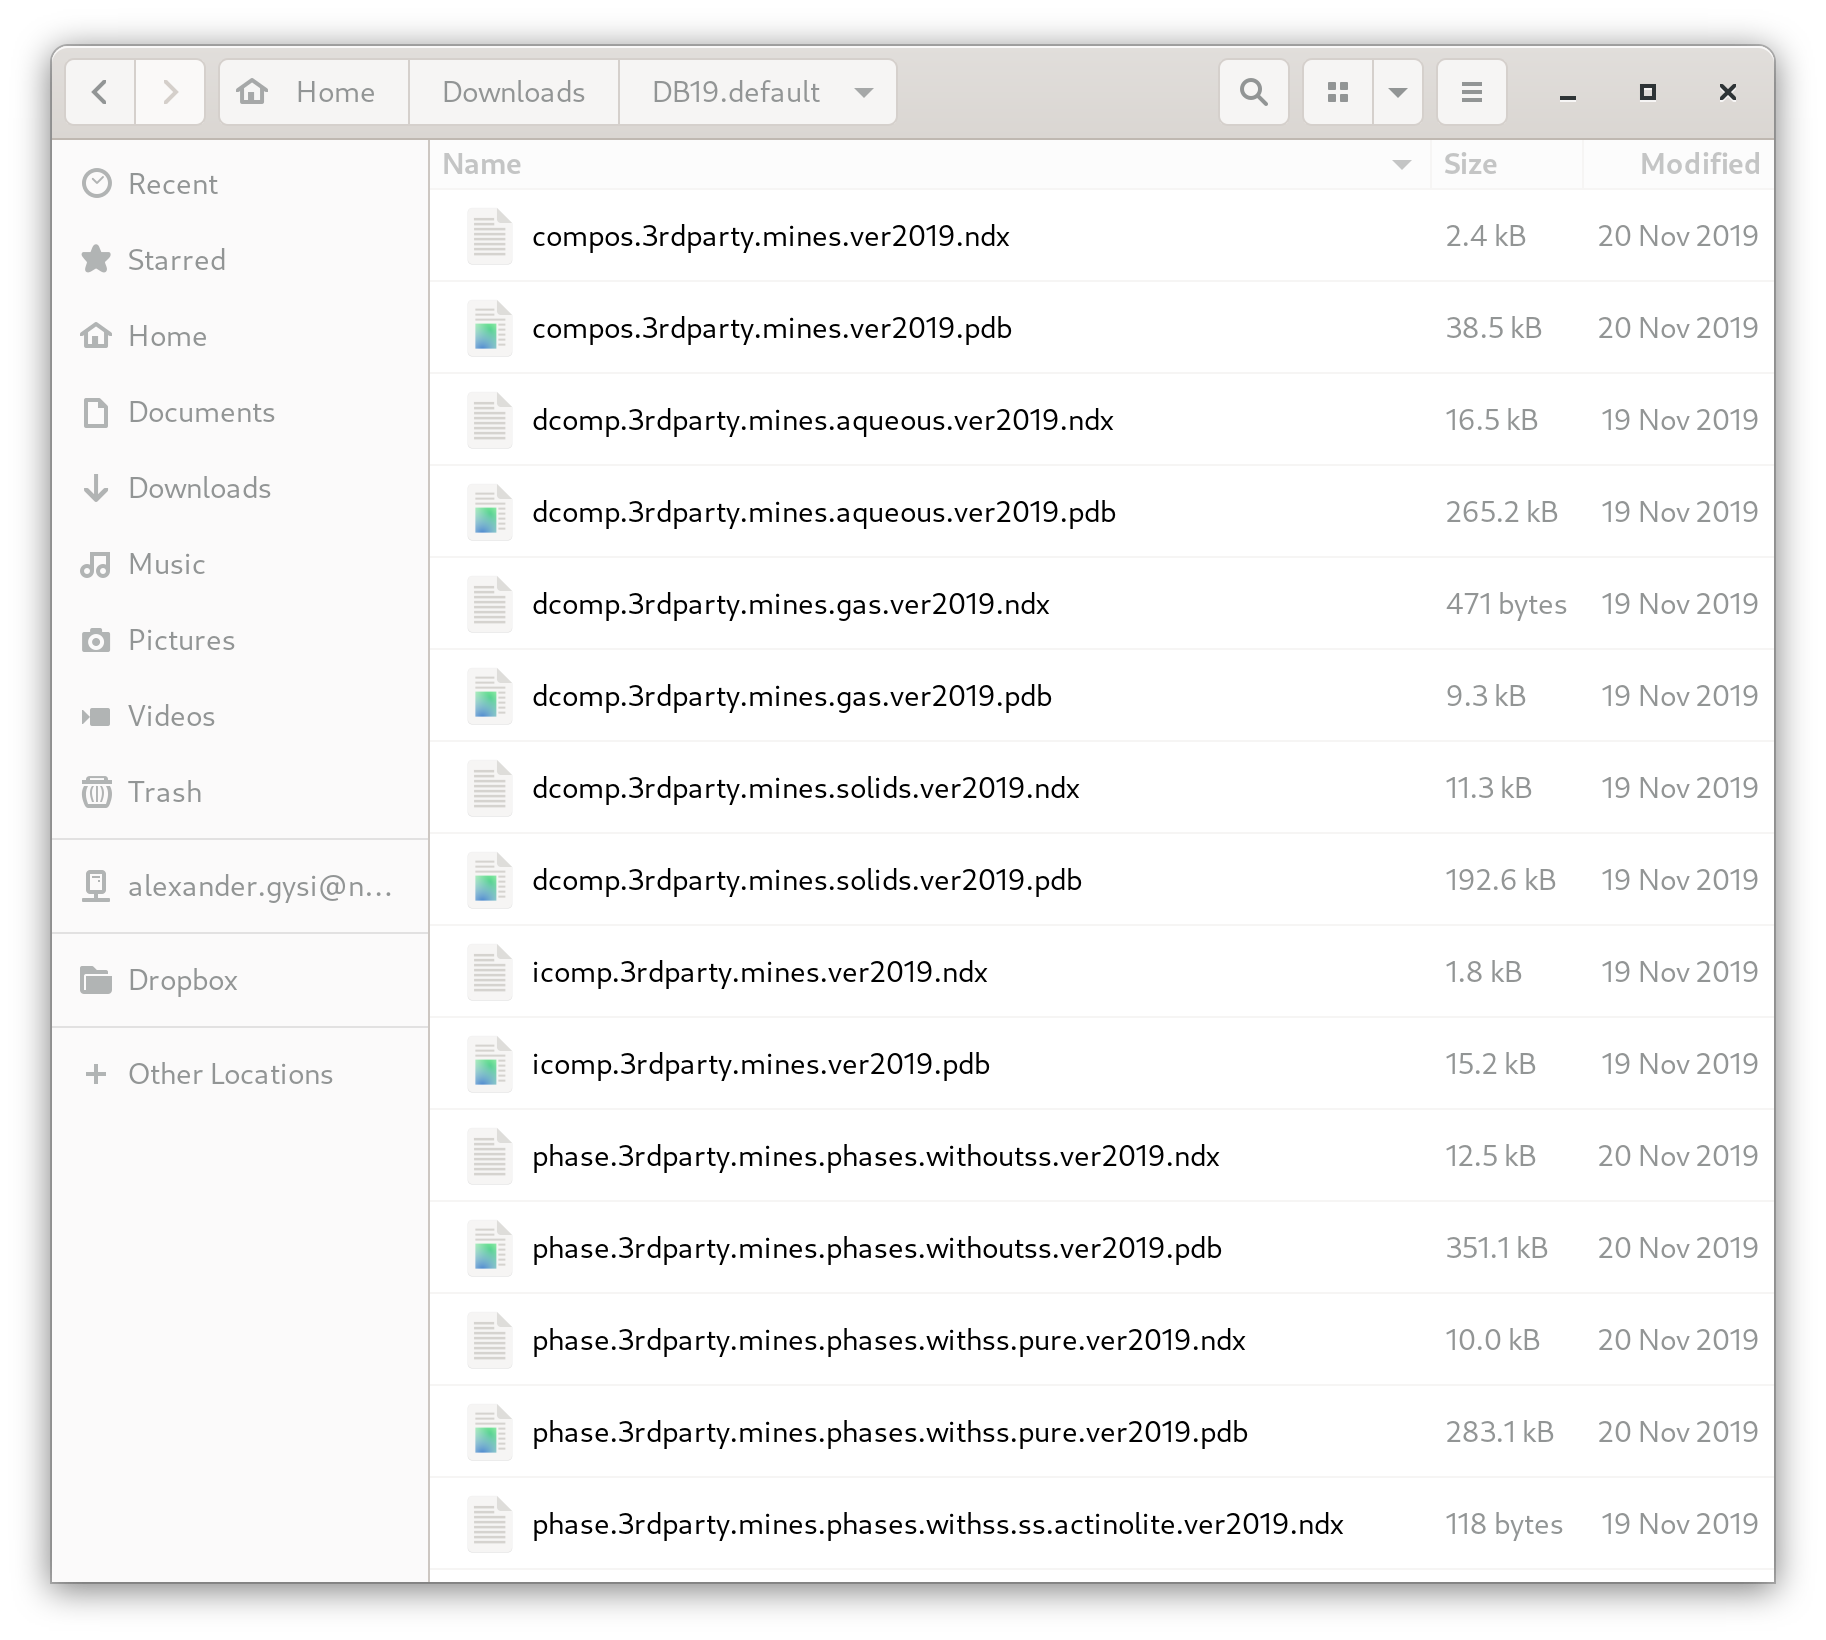
\includegraphics[width=0.7\linewidth]{figures/module1/fig-2} \caption{Unzipped DB19.default folder and database files to copy.}\label{fig:fig-2}
 \end{figure}

\begin{figure}
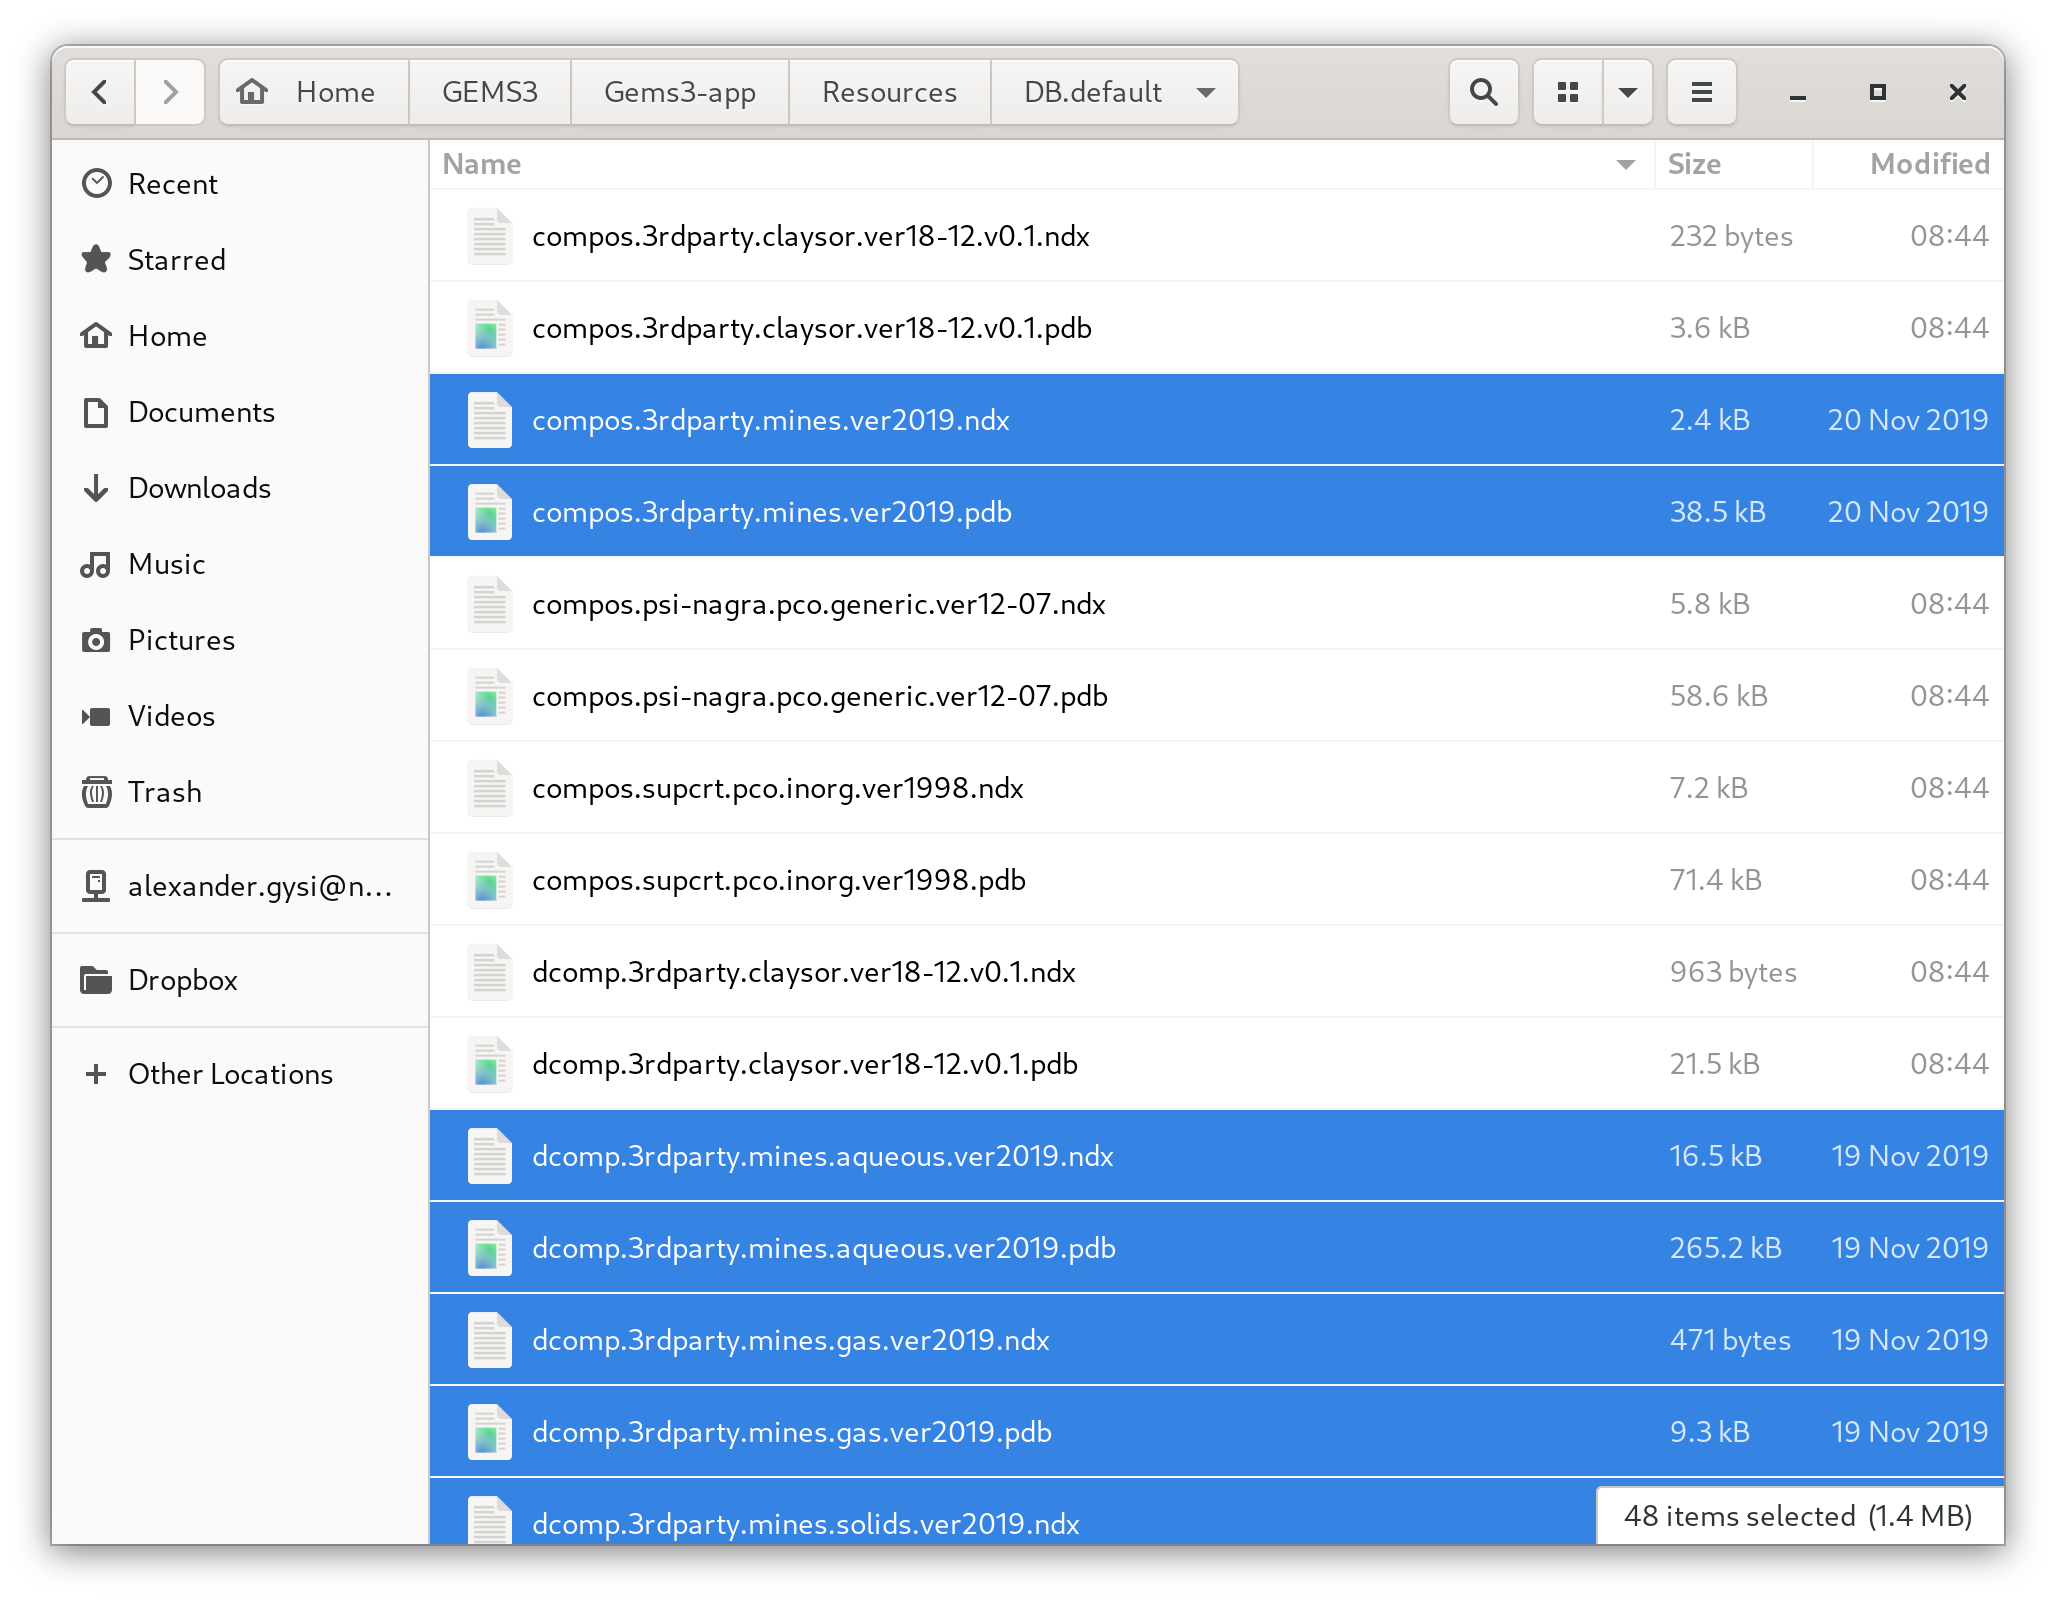
\includegraphics[width=0.7\linewidth]{figures/module1/fig-3} \caption{Database files merged with the Gems3-app/Resources/DB.default folder in GEMS.}\label{fig:fig-3}
\end{figure}

\hypertarget{creating-a-new-project-from-scratch}{%
\section{Creating a new project from scratch}\label{creating-a-new-project-from-scratch}}

\begin{itemize}
\item
  Open GEMS and click \texttt{New\ Project} in the Modeling Projects window. Give a name to your project (no spaces). The user interface is shown in Figure \ref{fig:fig-4}.
\item
  In the next window, you can choose the thermodynamic database for your project. Select the database files 3rdparty/MINES and support, then deselect other databases as shown in Figure \ref{fig:fig-5}. Click \texttt{Next}.
\end{itemize}

\emph{Do not forget, you have an extensive list of minerals included in this database. Once you have gone through the tutorials and are familiar with GEMS, it is suggested that in thermodynamic database mode you switch to the \texttt{Phase} module (Fig. \ref{fig:fig-9}), and remove minerals that are not relevant for your own specific project. Also, for less advanced users, it is easiedt to not use the ternary non-ideal feldspar solid solution model (ss) but only their end members (i.e., anorthite, albite and microcline).}

\begin{figure}
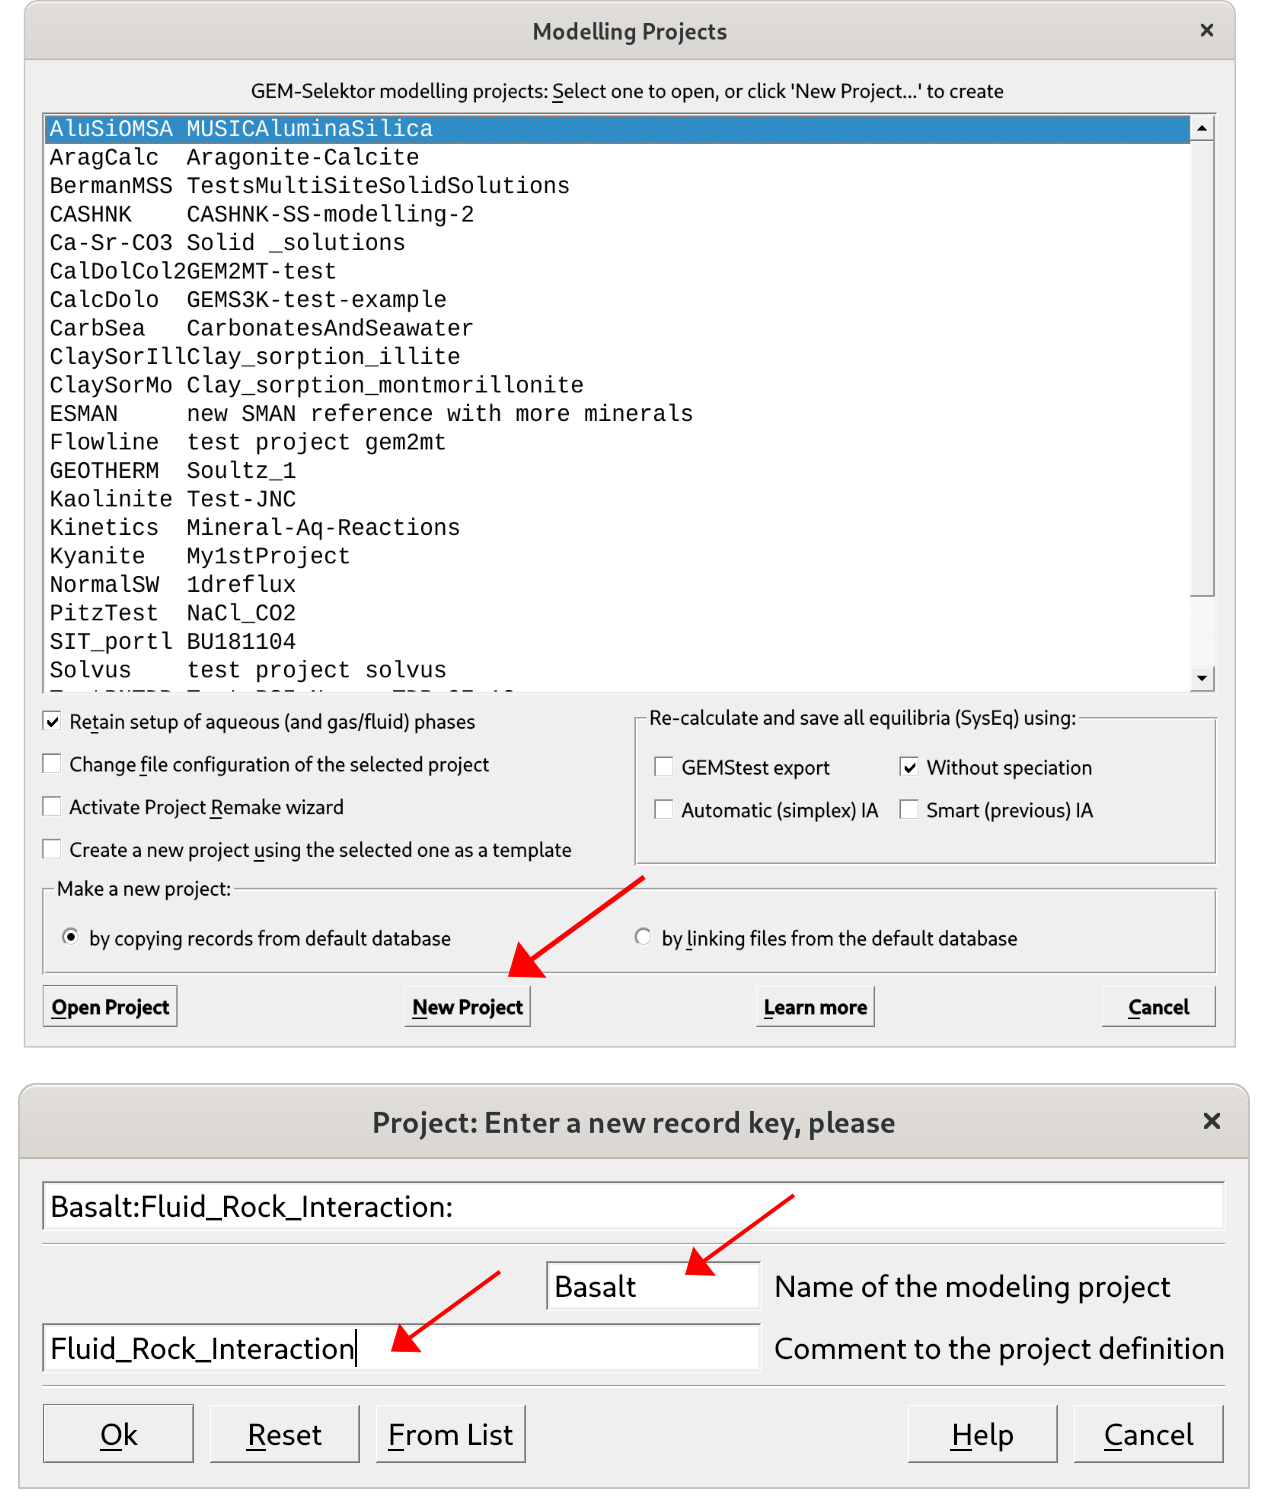
\includegraphics[width=0.7\linewidth]{figures/module1/fig-4} \caption{GEMS user interface showing the project window. Click on make a `New Project` and select a project name without spaces.}\label{fig:fig-4}
\end{figure}

\textbackslash begin\{figure\}
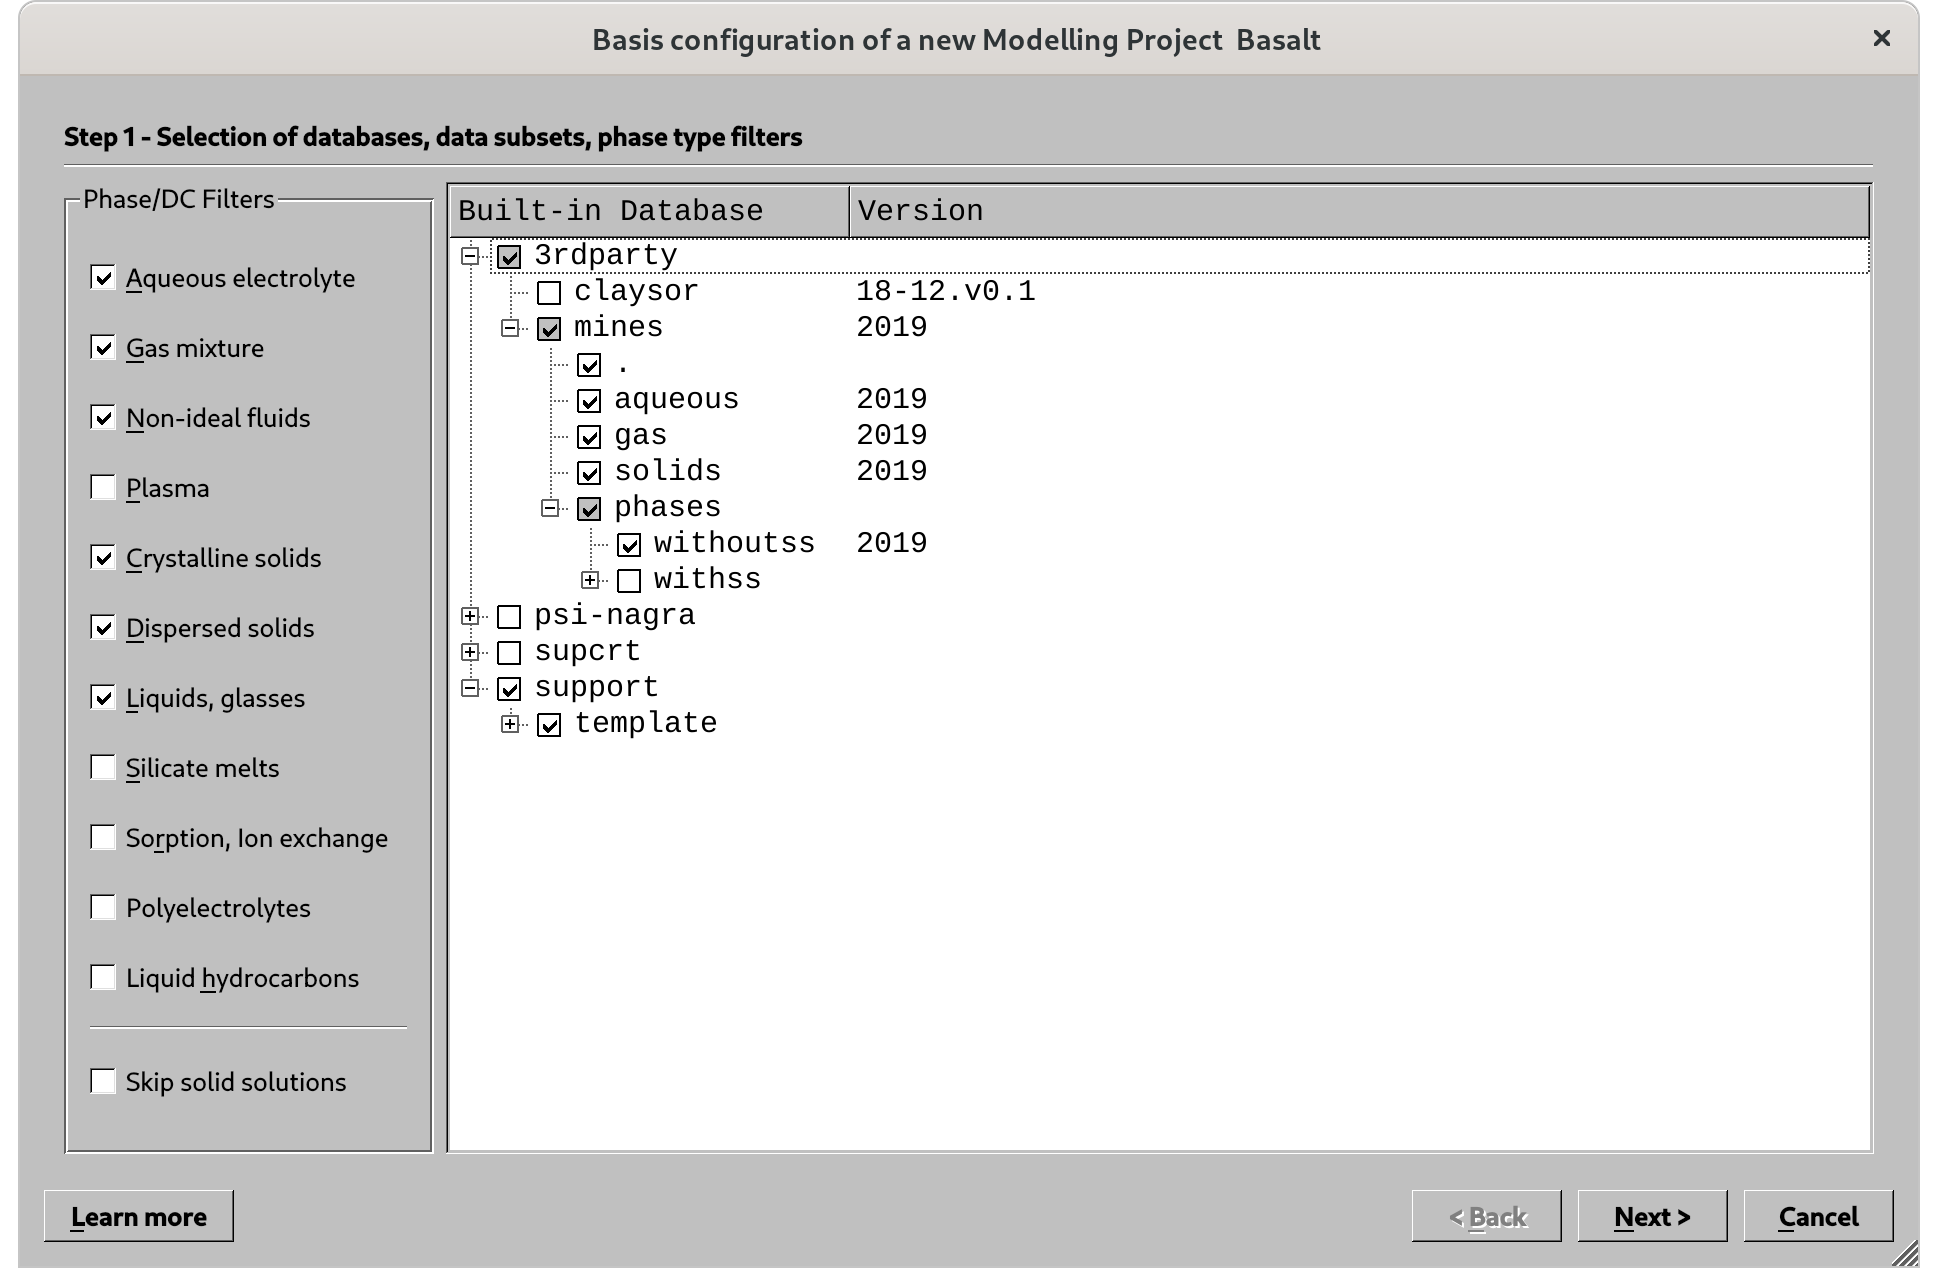
\includegraphics[width=0.7\linewidth]{figures/module1/fig-5} \textbackslash caption\{Select 3rdparty/mines and support, and for phases select only withoutss. \emph{Note that we recommend only advanced users to choose withss; the expanded tab shows pure for endmembers and ss for different solid solution endmembers}\}\label{fig:fig-5}
\textbackslash end\{figure\}

\begin{itemize}
\item
  In the next window choose your system components: H-O-C-Cl-Na-K-Ca-Mg-Al-Fe-Si-Ti (Fig. \ref{fig:fig-6}). Have you checked you got all of the elements selected? Check again please, then click \texttt{Next}\ldots By doing so, GEMS will automatically look up all phases with these components in the MINES database and copy them into your modeling project! \emph{Tip of the day: all your modeling projects you are working on are located under Library/Gems3/projects. Make sure to do regular backups\ldots{}}
\item
  In the next window you will be able to choose the activity model for your aqueous speciation calculations (e.g.~``Debye-Hückel'', Davies equation, \ldots), and the EOS for gases. For now, follow Figure \ref{fig:fig-7} using the extended ``Debye-Hückel'' equation (Helgeson), check the parameters and click \texttt{Check} for the aqueous speciation model. \emph{This model is ideal for modeling H\(_2\)O-NaCl aqueous solutions (with NaCl as background electrolyte) at hydrothermal conditions at relatively moderate salinities observed in many ore deposits.}
\item
  Then you can switch to the gas EOS model tab and choose the Peng-Robinson-Stryjek-Vera (PRSV) model and click \texttt{Check} (Fig. \ref{fig:fig-7}). That's it, now you are ready to model your first equilibrium model!
\end{itemize}

\emph{Note: this model is for non-ideal gases, and for this purpose a new phase with the acronym (f) was added to the MINES database with all the relevant parameters using the PRSV EOS. Else the choice would be the ideal gas law with a phase using the acronym (g)}

\begin{figure}
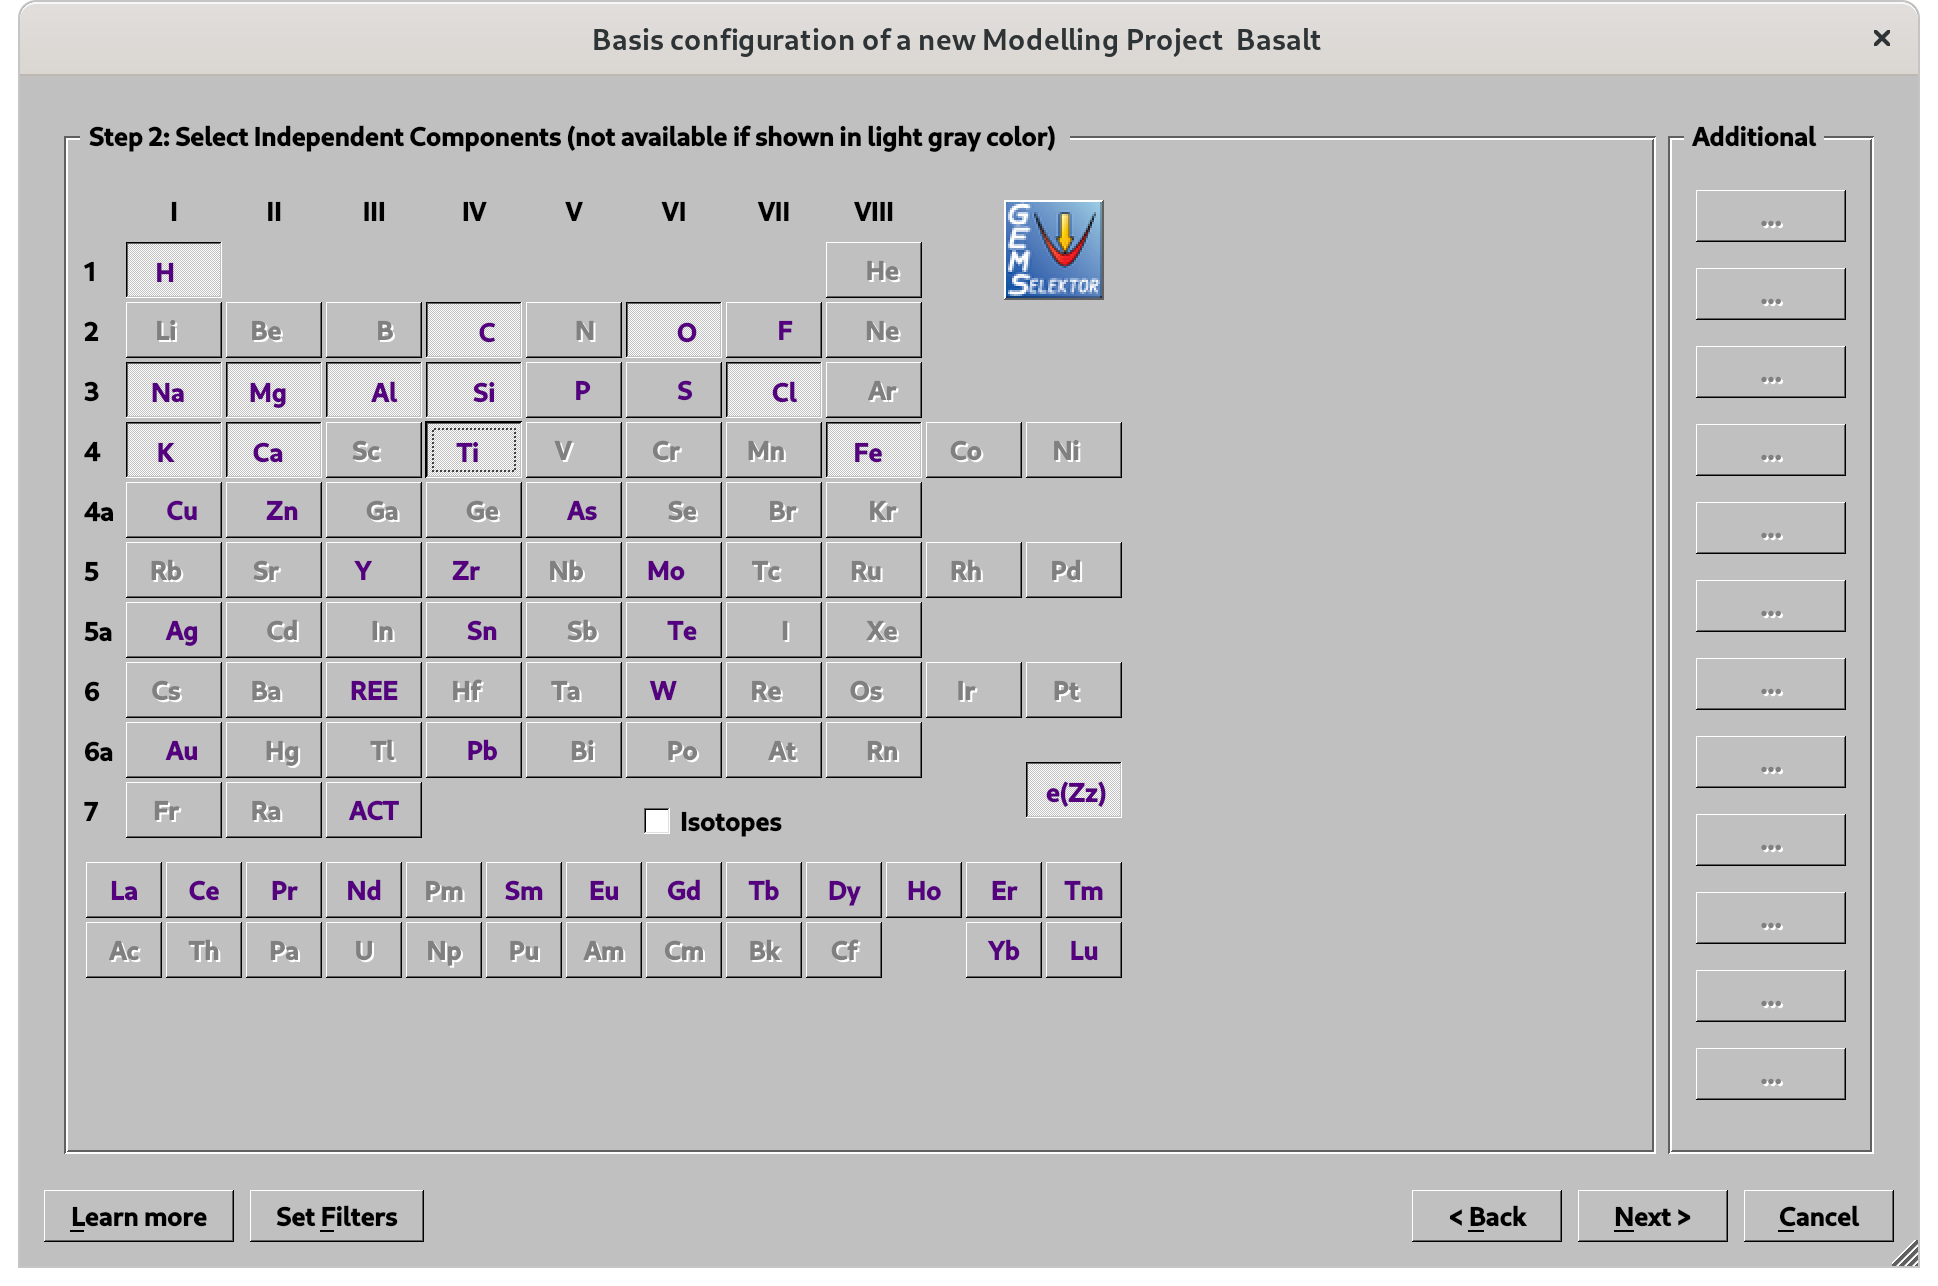
\includegraphics[width=0.8\linewidth]{figures/module1/fig-6} \caption{Select here the composition of the system. All phases containing these elements will automatically be loaded from the MINES database into your project.}\label{fig:fig-6}
\end{figure}

\begin{figure}
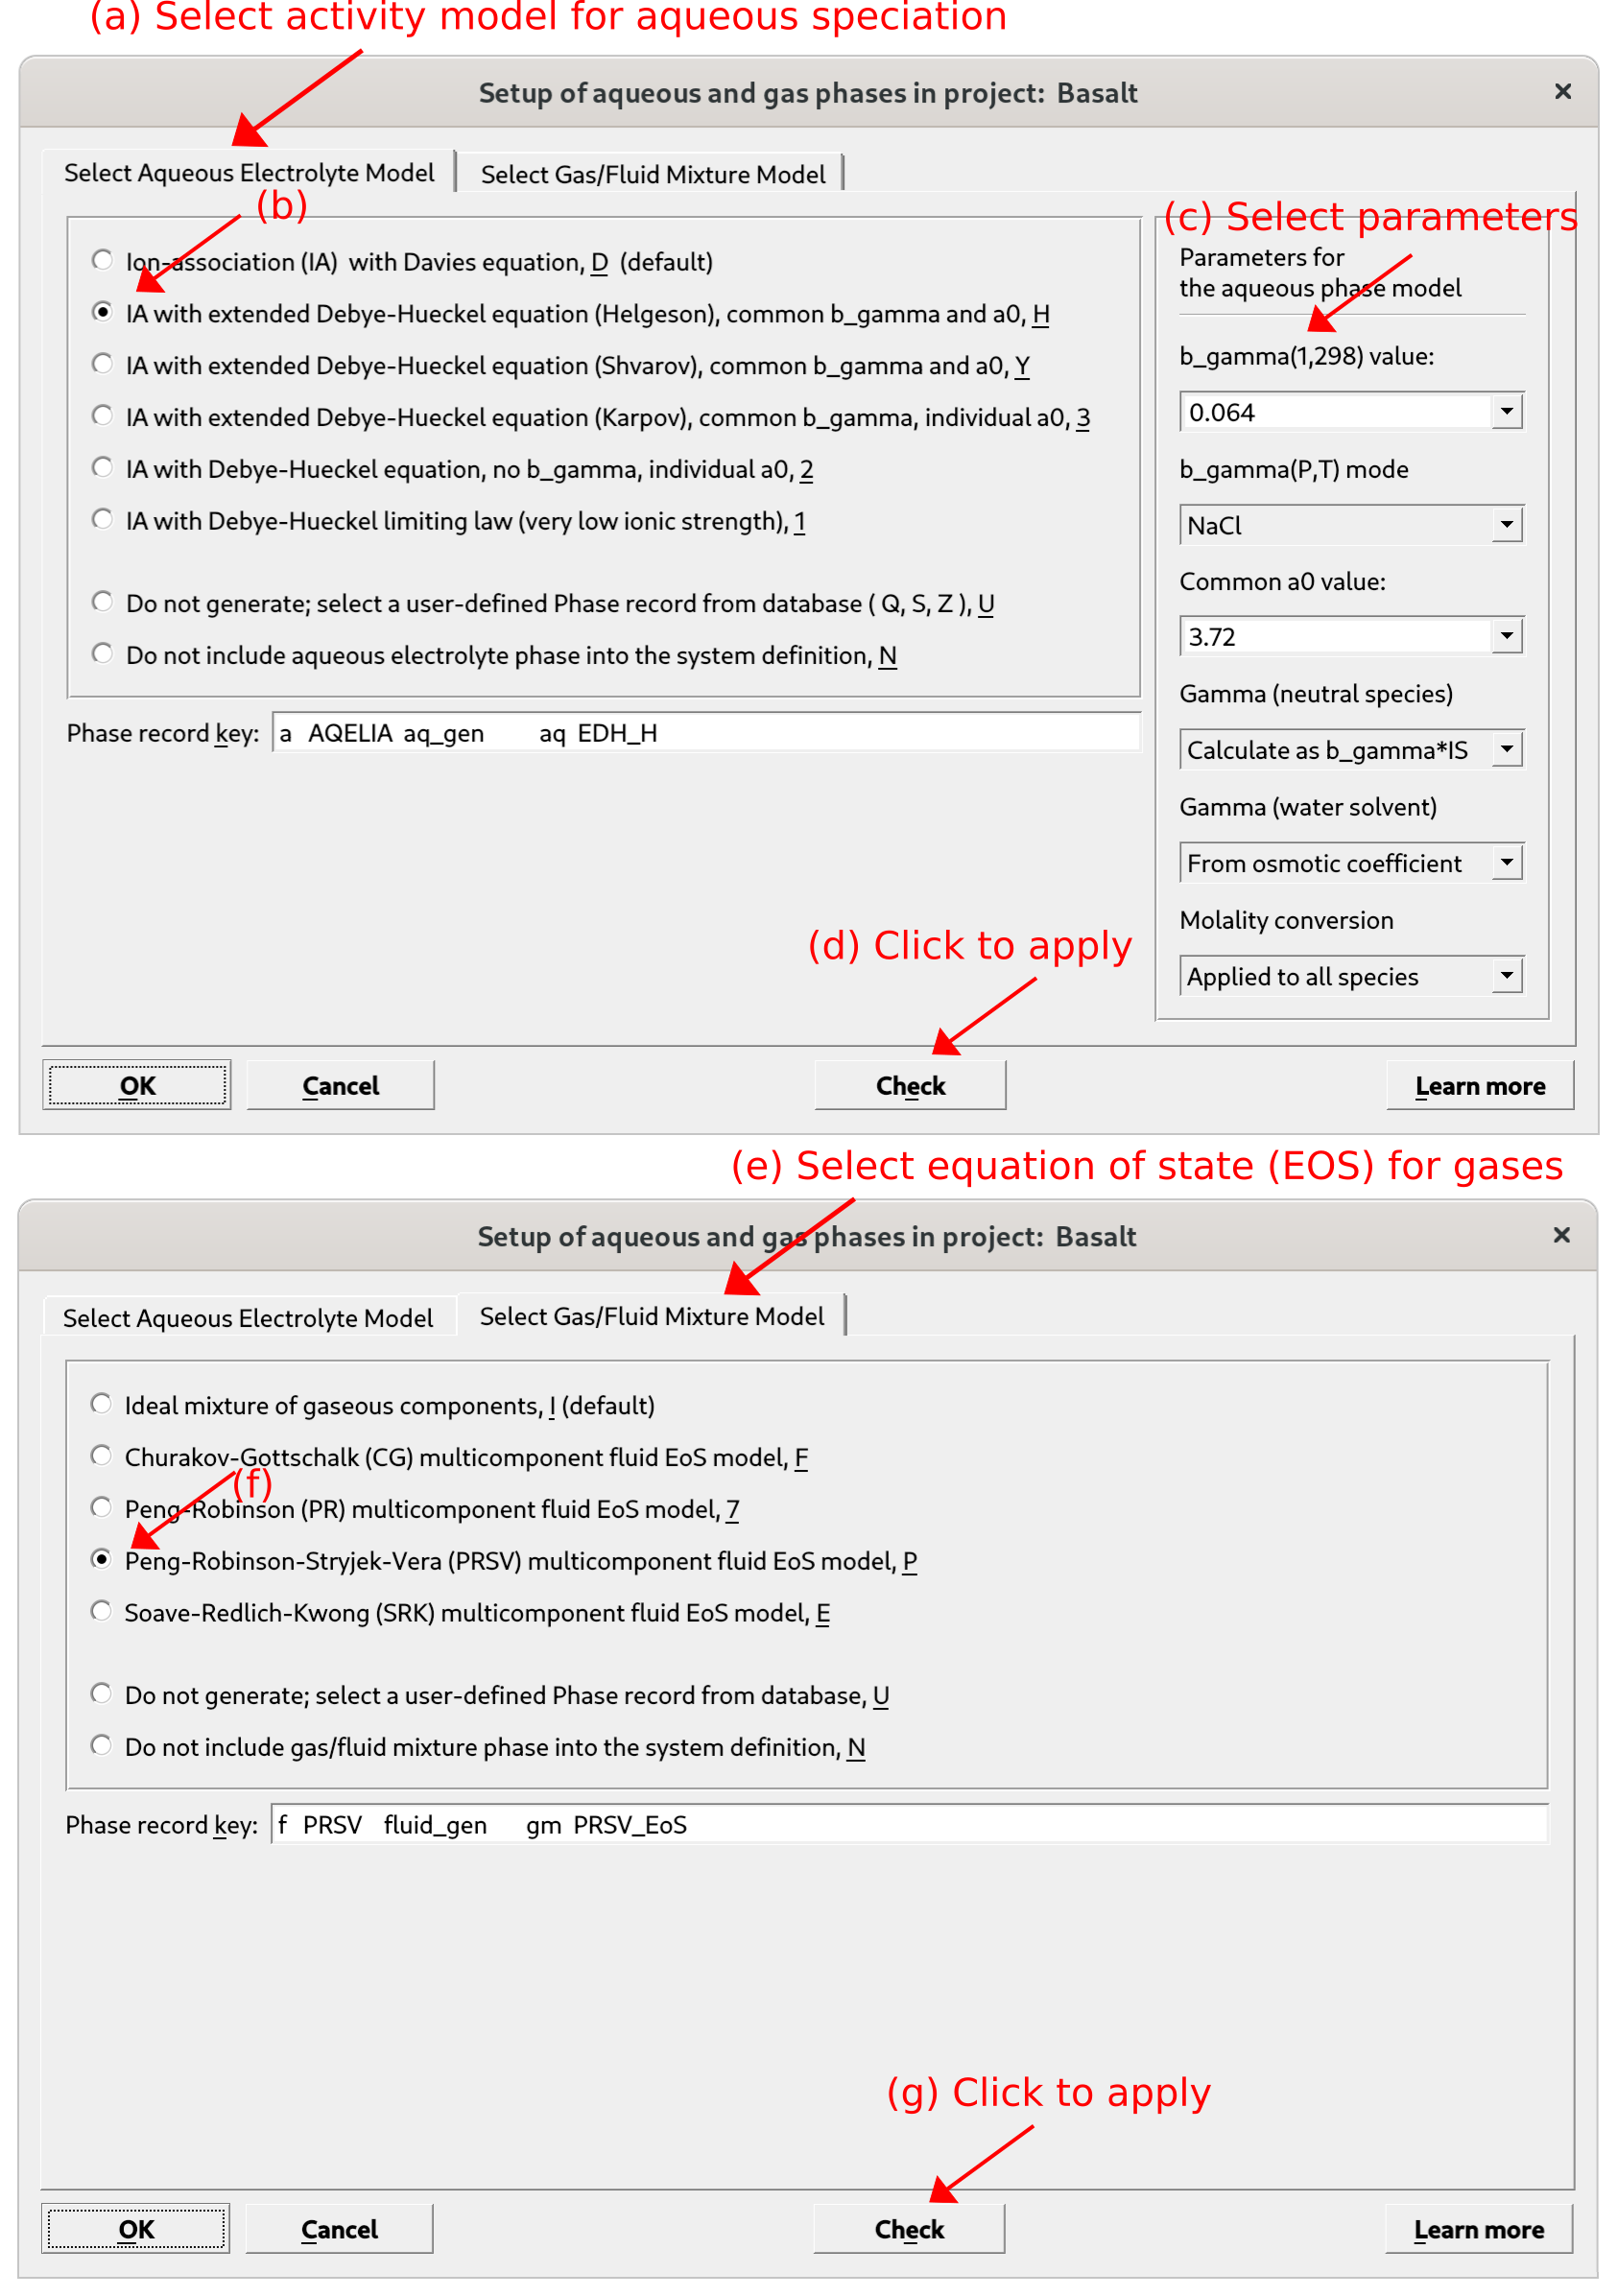
\includegraphics[width=0.7\linewidth]{figures/module1/fig-7} \caption{Select here the activity model for aqueous speciation (a-d) and the EOS model for gases (e-g).}\label{fig:fig-7}
\end{figure}

\hypertarget{your-first-fluid-rock-equilibrium-model}{%
\section{Your first fluid-rock equilibrium model}\label{your-first-fluid-rock-equilibrium-model}}

\begin{itemize}
\item
  In the next window, you will be able to define the name of your first fluid-rock system equilibrium (\texttt{SysEq}) calculations and set the pressure and temperature (Fig. \ref{fig:fig-8}).
\item
  Add a name without spaces and P-T conditions, i.e.~we choose basalt-fluid, 250 \(^{\circ}\)C for T and 1 kbar for P.
\item
  Next window we select our ingredients and add 1000 g of H\(_2\)O (Aqua), 200 g of NaCl, 5 g Gas CO\(_2\) and 500 g of basalt (Fig. \ref{fig:fig-8}). Click \texttt{OK}.
\item
  Finally, you can click on \texttt{Calculate\ BCC} followed by \texttt{Calculate\ equilibrium\ with\ GEM} as shown in (Fig. \ref{fig:fig-9}). You can easily create another system by selecting \texttt{Clone\ a\ new\ record\ from\ this\ one} and change the fluid/rock ratio or temperature and see what what happens with the results.
\end{itemize}

\begin{figure}
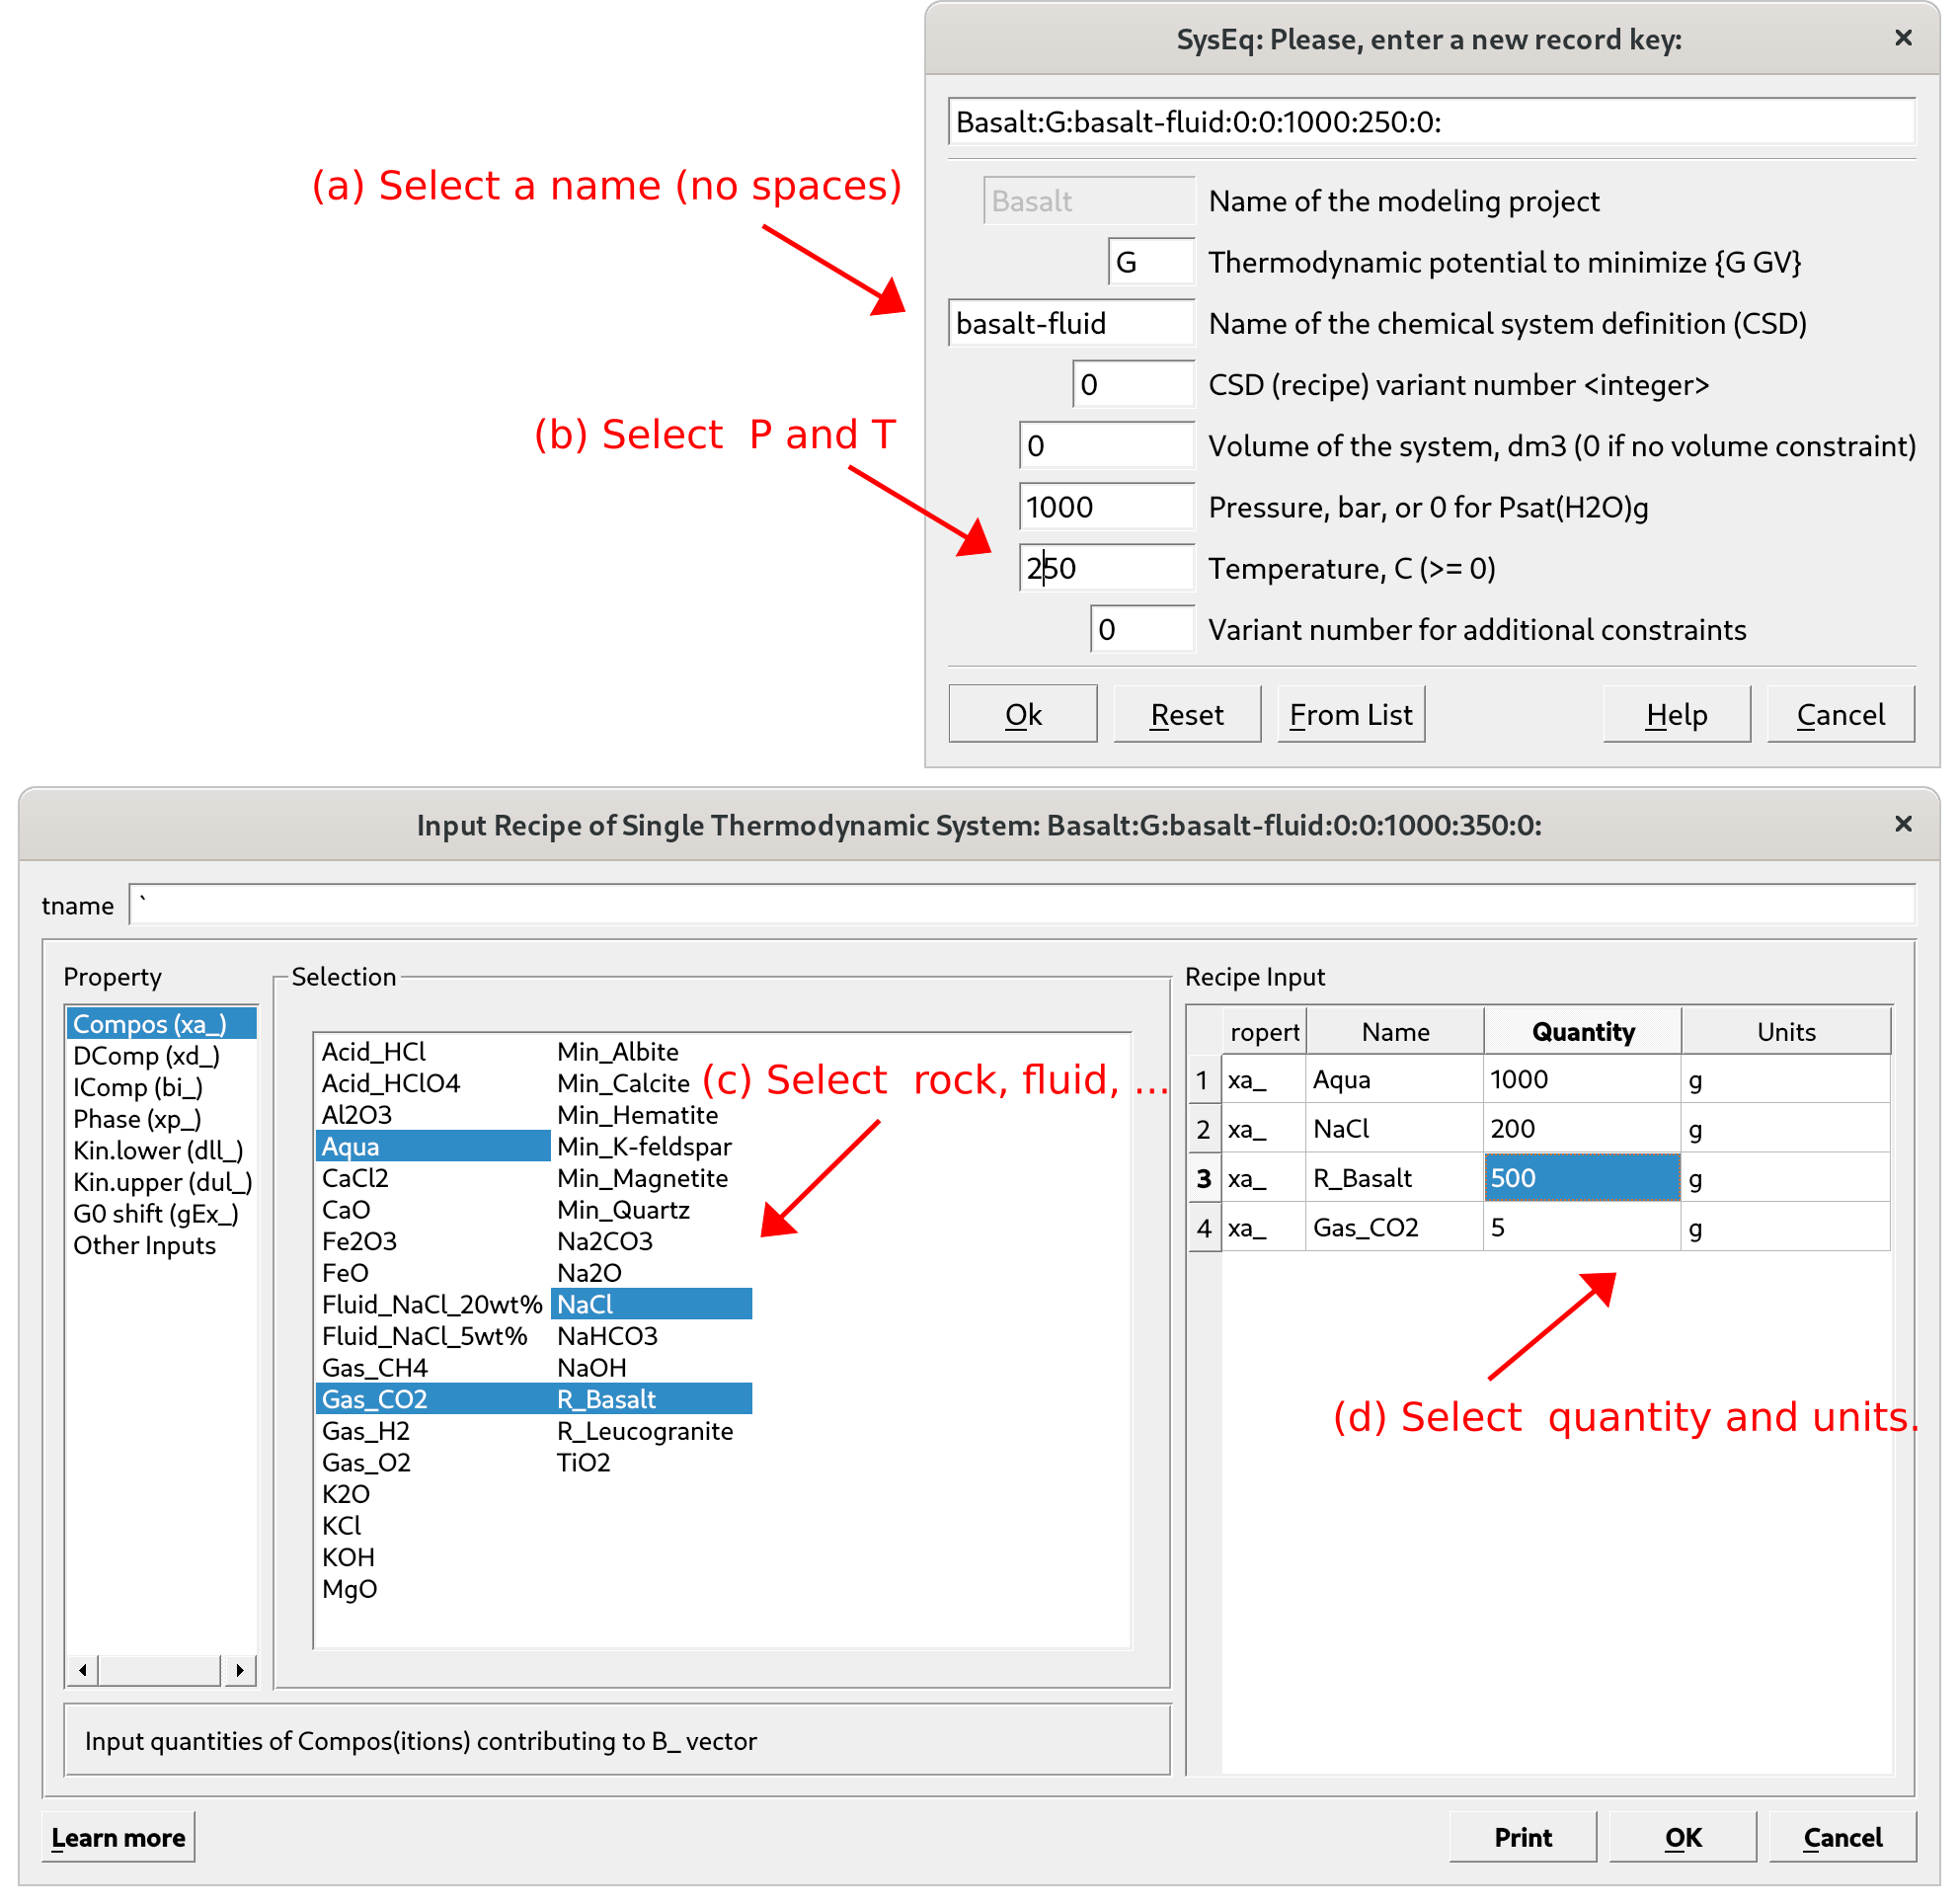
\includegraphics[width=0.7\linewidth]{figures/module1/fig-8} \caption{GEM-Selektor user interface showing the windows to create a new equilibrium system and define pressure (P) and temperature (T) for our first calculation.}\label{fig:fig-8}
\end{figure}

\begin{figure}
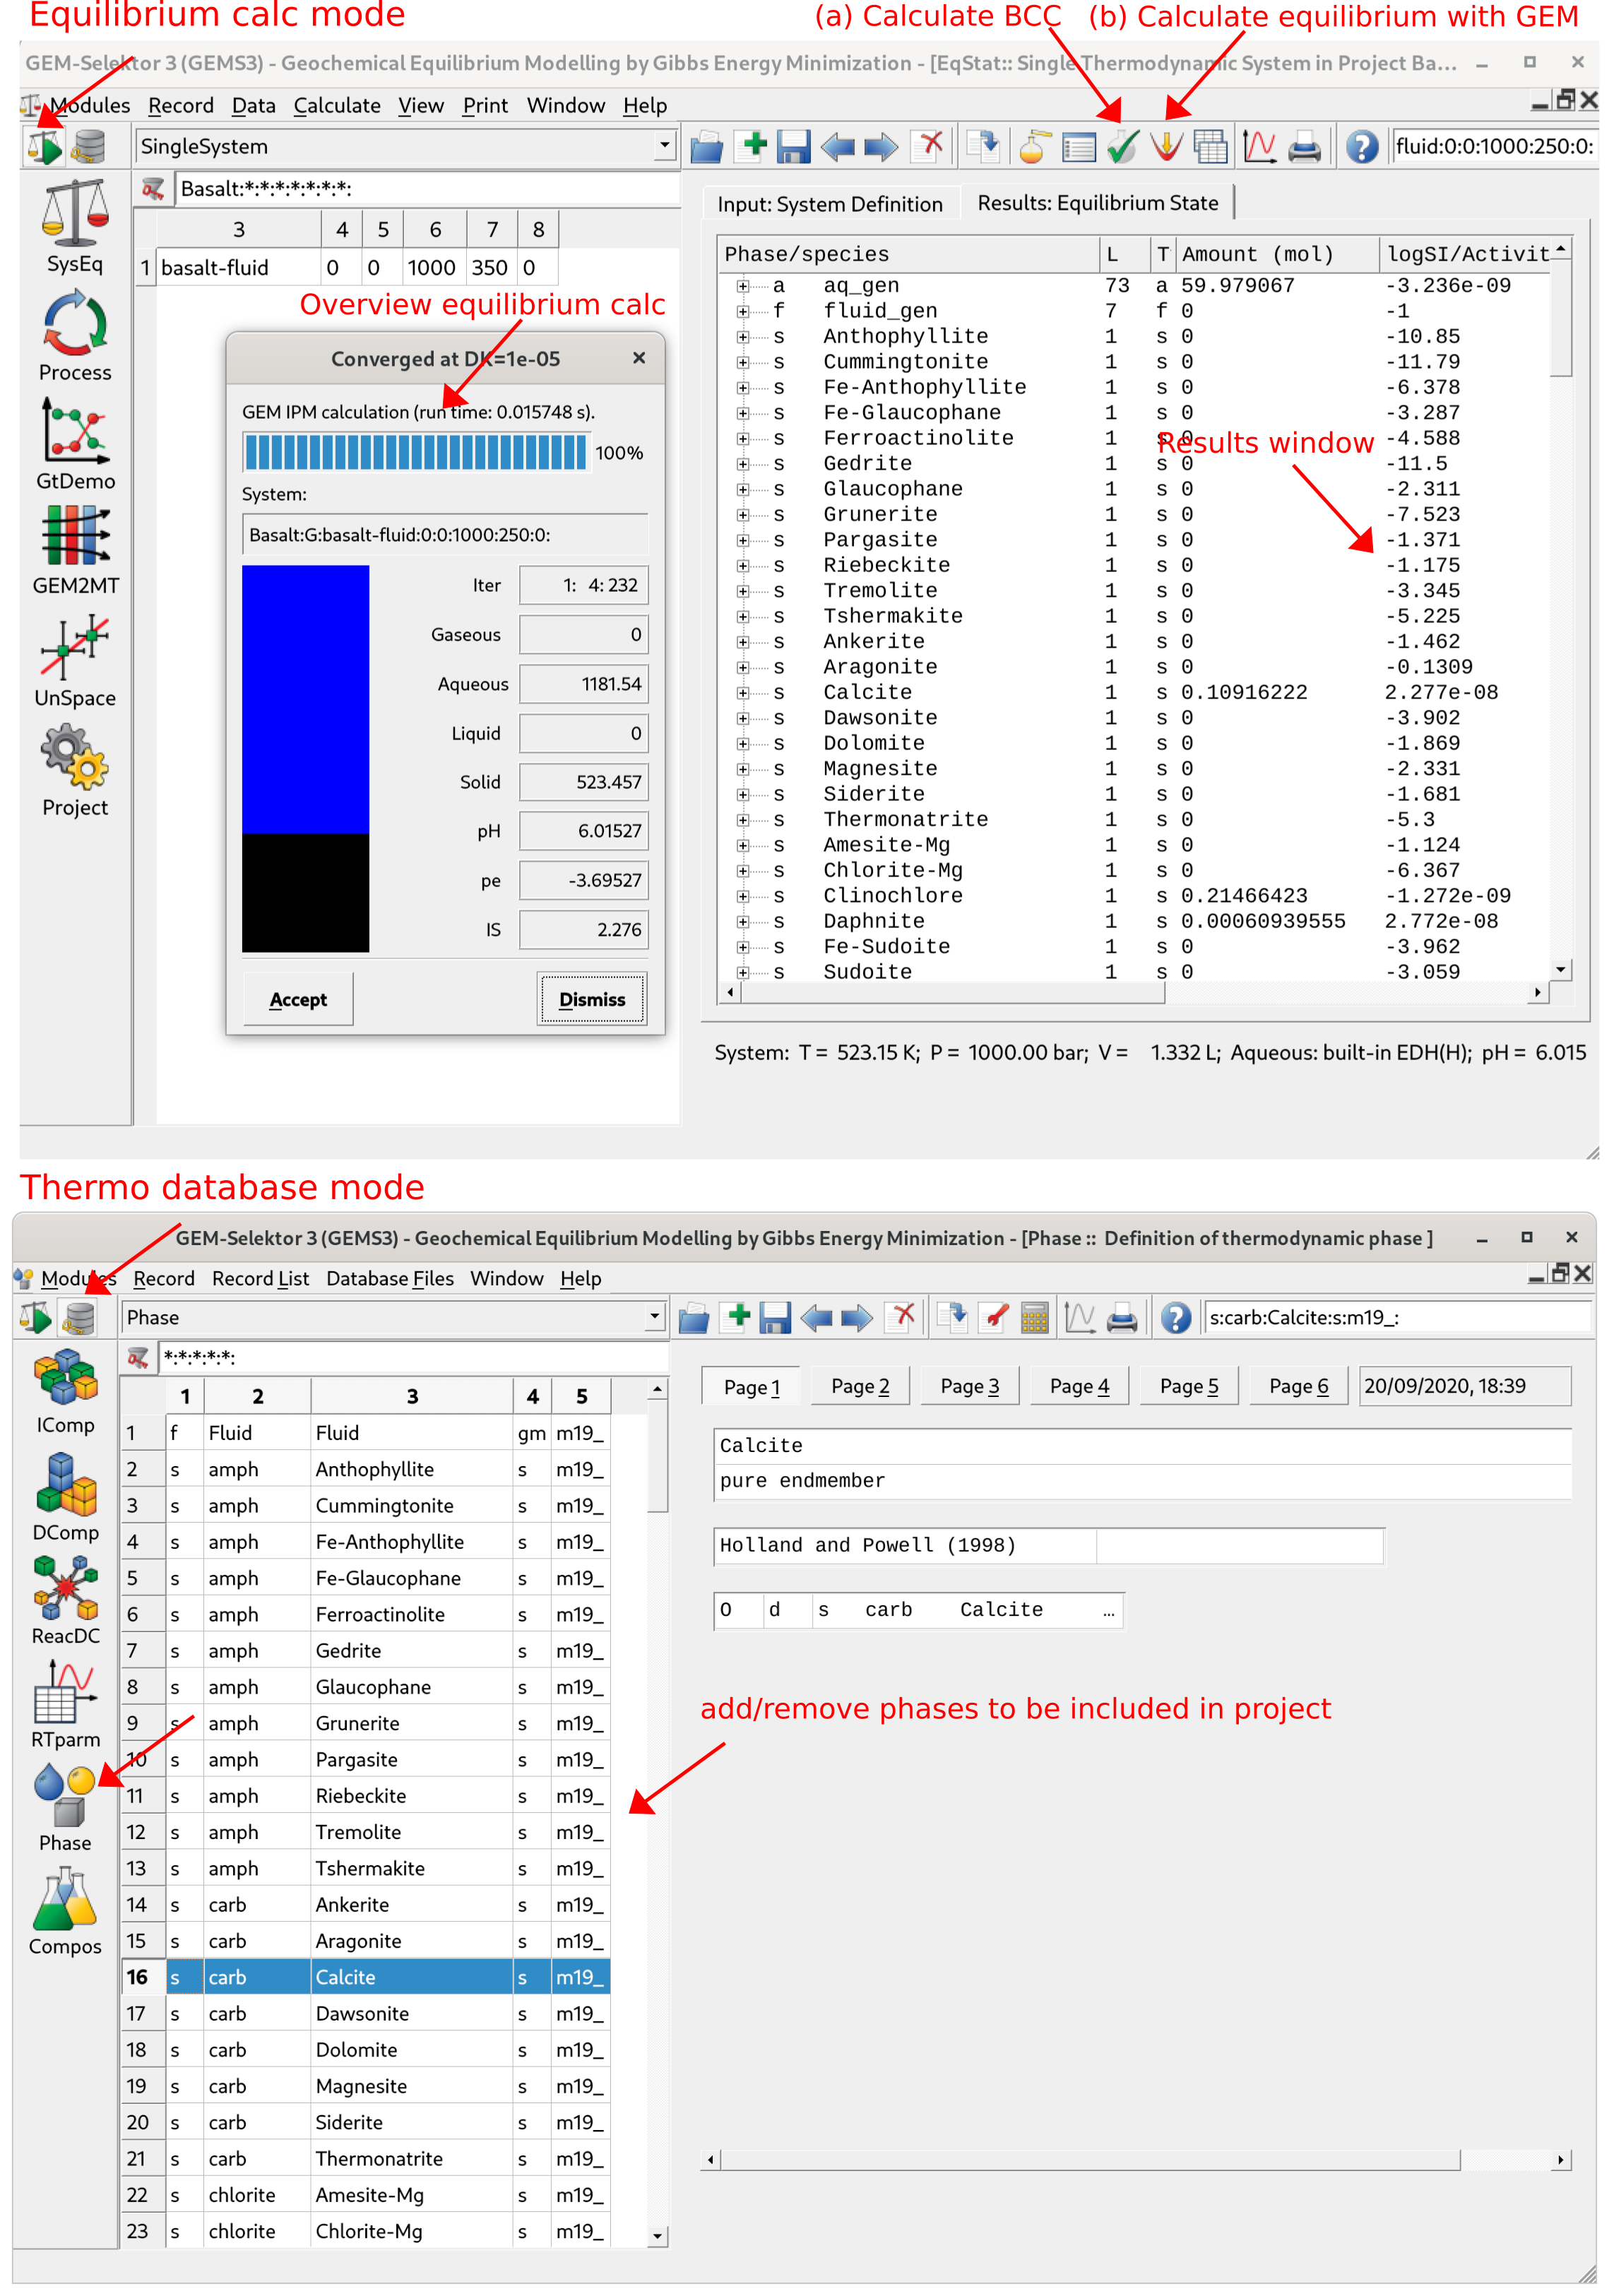
\includegraphics[width=0.7\linewidth]{figures/module1/fig-9} \caption{GEM-Selektor user interface showing how to `Calculate BCC` followed by `Calculate equilibrium with GEMS`. Also shown are the `Equilibrium Calculation` mode and the `Thermodynamic database` mode, where you can inspect the MINES database.}\label{fig:fig-9}
\end{figure}

\hypertarget{outcomes}{%
\section{Outcomes}\label{outcomes}}

Congratulations! In Module 1 you learned how to install the MINES thermodynamic database in your Resources/DB.default GEMS folder, the general folder structure of GEMS, how to setup your first project and how to run your first fluid-rock equilibrium calculations in GEMS.

\hypertarget{module-2}{%
\chapter{Module 2}\label{module-2}}

Work in progress\ldots{}

\hypertarget{module-3}{%
\chapter{Module 3}\label{module-3}}

Work in progress\ldots{}

\hypertarget{module-4}{%
\chapter{Module 4}\label{module-4}}

Work in progress\ldots{}

\hypertarget{module-5}{%
\chapter{Module 5}\label{module-5}}

Work in progress\ldots{}

  \bibliography{book.bib,packages.bib}

\end{document}
